% THIS IS SIGPROC-SP.TEX - VERSION 3.1
% WORKS WITH V3.2SP OF ACM_PROC_ARTICLE-SP.CLS
% APRIL 2009
%
% It is an example file showing how to use the 'acm_proc_article-sp.cls' V3.2SP
% LaTeX2e document class file for Conference Proceedings submissions.
% ----------------------------------------------------------------------------------------------------------------
% This .tex file (and associated .cls V3.2SP) *DOES NOT* produce:
%       1) The Permission Statement
%       2) The Conference (location) Info information
%       3) The Copyright Line with ACM data
%       4) Page numbering
% ---------------------------------------------------------------------------------------------------------------
% It is an example which *does* use the .bib file (from which the .bbl file
% is produced).
% REMEMBER HOWEVER: After having produced the .bbl file,
% and prior to final submission,
% you need to 'insert'  your .bbl file into your source .tex file so as to provide
% ONE 'self-contained' source file.
%
% Questions regarding SIGS should be sent to
% Adrienne Griscti ---> griscti@acm.org
%
% Questions/suggestions regarding the guidelines, .tex and .cls files, etc. to
% Gerald Murray ---> murray@hq.acm.org
%
% For tracking purposes - this is V3.1SP - APRIL 2009

\documentclass{sig-alternate}
\usepackage{amstext}
\usepackage{pdfpages}
\usepackage{alltt}
\usepackage{epstopdf}
\usepackage{xspace,colortbl}
\usepackage[USenglish]{babel}
\usepackage{multirow}
\usepackage{url}
\usepackage{subfigure}
\usepackage{graphicx}
\usepackage{amssymb}
\usepackage{fmtcount}
\usepackage{amsfonts}
\usepackage{xspace}
\usepackage{amsmath}
\usepackage{multirow}
\usepackage[mathscr]{eucal}
%\usepackage{psfrag}
\usepackage{colortbl}
\usepackage{bm}
\usepackage[nospace]{cite}
\makeatletter
\newif\if@restonecol
\makeatother
\let\algorithm\relax
\let\endalgorithm\relax
\usepackage[lined,boxed,vlined,ruled]{algorithm2e}
\usepackage[skip=1pt,font=bf]{caption}
\special{papersize=8.5in,11in}


%\makeatletter
%\def\@copyrightspace{\relax}
%\makeatother

\newfont{\mycrnotice}{ptmr8t at 7pt}
\newfont{\myconfname}{ptmri8t at 7pt}
\let\crnotice\mycrnotice%
\let\confname\myconfname%

\permission{Permission to make digital or hard copies of all or part of this work for personal or classroom use is granted without fee provided that copies are not made or distributed for profit or corecsysercial advantage and that copies bear this notice and the full citation on the first page. Copyrights for components of this work owned by others than the author(s) must be honored. Abstracting with credit is permitted. To copy otherwise, or republish, to post on servers or to redistribute to lists, requires prior specific permission and/or a fee. Request permissions from permissions@acm.org.}
\conferenceinfo{RecSys'14,}{October 6--10, 2014, Foster City, Silicon Valley, CA, USA. \\
{\mycrnotice{Copyright is held by the owner/author(s). Publication rights licensed to ACM.}}}
\copyrightetc{ACM \the\acmcopyr}
\crdata{ACM 978-1-4503-2668-1/14/10\$15.00}

\clubpenalty=10000 
\widowpenalty = 10000

\begin{document}

\title{A Methodology for Learning, Analyzing, and Mitigating Social Influence Bias in Recommender Systems}

\linespread{0.945}%
\setlength{\belowdisplayskip}{2pt} \setlength{\belowdisplayshortskip}{2pt}
\setlength{\abovedisplayskip}{2pt} \setlength{\abovedisplayshortskip}{2pt}
\setlength{\belowcaptionskip}{-8pt}
\selectfont

%
% You need the command \numberofauthors to handle the 'placement
% and alignment' of the authors beneath the title.
%
% For aesthetic reasons, we recommend 'three authors at a time'
% i.e. three 'name/affiliation blocks' be placed beneath the title.
%
% NOTE: You are NOT restricted in how many 'rows' of
% "name/affiliations" may appear. We just ask that you restrict
% the number of 'columns' to three.
%
% Because of the available 'opening page real-estate'
% we ask you to refrain from putting more than six authors
% (two rows with three columns) beneath the article title.
% More than six makes the first-page appear very cluttered indeed.
%
% Use the \alignauthor commands to handle the names
% and affiliations for an 'aesthetic maximum' of six authors.
% Add names, affiliations, addresses for
% the seventh etc. author(s) as the argument for the
% \additionalauthors command.
% These 'additional authors' will be output/set for you
% without further effort on your part as the last section in
% the body of your article BEFORE References or any Appendices.

\numberofauthors{1} %  in this sample file, there are a *total*
\author{ Sanjay Krishnan, Jay Patel, Michael J. Franklin, Ken Goldberg\\
\affaddr{Department of Electrical Engineering and Computer Sciences, UC Berkeley} \\
\email{\{sanjaykrishnan, patel.jay, franklin, goldberg\}@berkeley.edu}\\
}
% of EIGHT authors. SIX appear on the 'first-page' (for formatting
% reasons) and the remaining two appear in the \additionalauthors section.
%\author{Sanjay Krishnan,Jay Patel,Ken Goldberg}

%

% Just remember to make sure that the TOTAL number of authors
% is the number that will appear on the first page PLUS the
% number that will appear in the \additionalauthors section.

\maketitle
\begin{abstract}
The seminal 2003 paper by Cosley, Lab, Albert, Konstan, and Reidl, demonstrated the 
susceptibility of recommender systems to rating biases.  
To facilitate browsing and selection, almost all recommender systems
display average ratings before accepting ratings from users which has been shown to bias ratings.
This effect is called Social Influence Bias (SIB); 
the tendency to conform to the perceived ``norm" in a community.
We propose a methodology to 1) learn, 2) analyze, and 3) mitigate the effect of
SIB in recommender systems.  In the Learning phase,
we build a baseline dataset by allowing users to rate twice: before and after seeing the average rating.  
In the Analysis phase, we apply a new non-parametric significance test based on the Wilcoxon statistic to
test whether the data is consistent with SIB.  
If significant, we propose a Mitigation phase using polynomial regression
and the Bayesian Information Criterion (BIC) to predict unbiased ratings.
We evaluate our approach on a dataset of 9390 ratings from the California Report Card (CRC), a 
rating-based system designed to encourage political engagement.
We found statistically significant evidence of SIB.
Mitigating models were able to predict changed ratings with a normalized RMSE of 12.8\% and 
reduce bias by 76.3\%.
The CRC, our data, and experimental code are available at:\\
http://californiareportcard.org/data/
\end{abstract}

% A category with the (minimum) three required fields
%\category{H.4}{Information Systems Applications}{Miscellaneous}
%A category including the fourth, optional field follows...
%\category{D.2.8}{Software Engineering}{Metrics}[complexity measures, performance measures]

%\terms{Theory}

%\keywords{ACM proceedings, \LaTeX, text tagging} % NOT required for Proceedings
\sloppy
% !TEX root = demo.tex
\section{Introduction}\label{sec:intro}

\begin{figure}[t]
\centering
\vspace{-0.5cm}
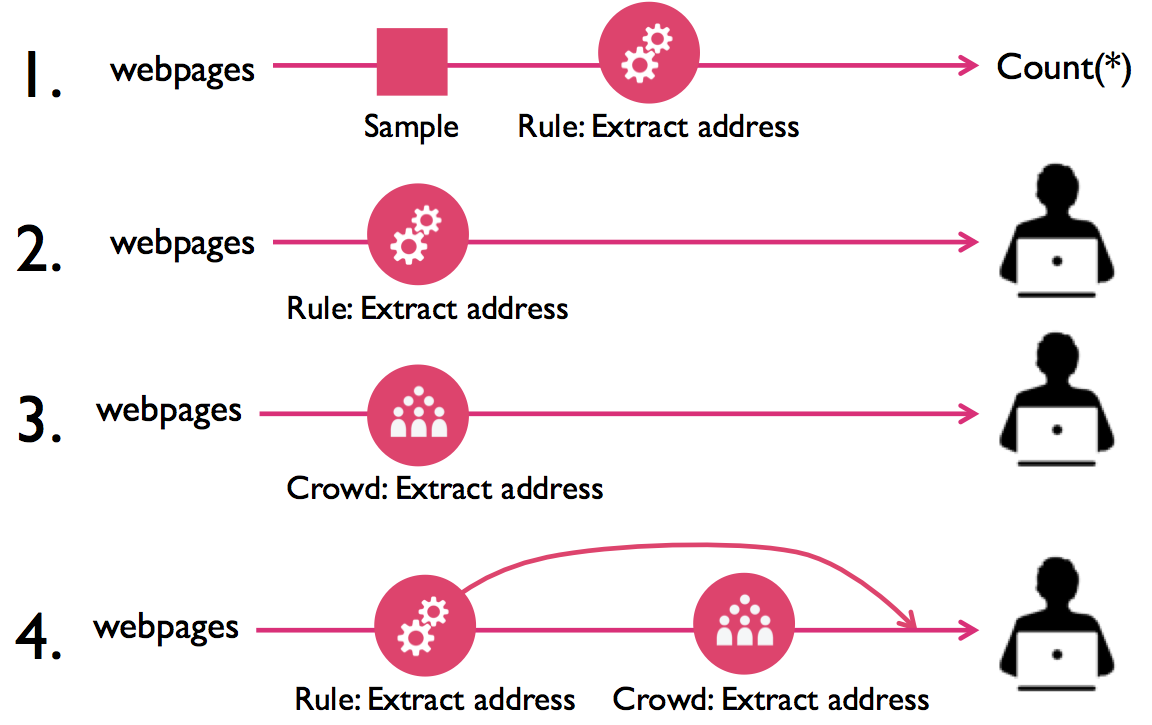
\includegraphics[width = .4\textwidth]{figs/lifecycle.png}
\vspace{-0.4cm}
\caption{Example iterations on the design of the portion of a cleaning plan that extracts restaurant addresses from their unstructured webpages.  
1) An exploratory plan that uses a sample to evaluate a simple address extraction method.
2) A plan that applies the method to the entire dataset. The quality is unsatisfactory. 
3) An alternate plan that uses manual crowd extraction. The quality is now high, but the crowd-based extractor is slow. 
4) A hybrid plan that sends only difficult webpages to the crowd, maximizing accuracy without sacrificing latency.}
\label{fig:ex-plan}
\vspace{-0.3cm}
\end{figure}
% why feedback loops exist/are important (cite Joe’s shit in the past 3 years, blinkdb, etc.). highlight domain specificity. Large variety of data cleaning tasks

%
% General comment that data cleaning is important:
%
The ease of acquiring and merging many large-scale data sources has led to a prevalence of dirty data.
Unfortunately, blindly using results that are derived from dirty data can lead to hidden yet significant errors in modern data-driven applications, so data must be cleaned before it is used.
But because data cleaning is often specific to the domain, dataset, and eventual analysis, analysts report spending upwards of 80\% of their time on problems in data cleaning~\cite{kandel2012}.
The analyst is faced with a breadth of possible errors that are manifest in the data and a variety of options to resolve them.
She must go through the cleaning process via trial and error, deciding for each of her data sources what to extract, how to clean it, and whether that cleaning will significantly change results.

Data cleaning is inherently iterative and Figure~\ref{fig:ex-plan} shows a common progression for the development of a data cleaning plan, in this case the extraction of a restaurant's address from its unstructured webpage.
While this operation can easily be represented at a \textit{logical} level by its input and output schema, there is a huge space of possible \textit{physical} implementations of the logical operators. 
For example, extraction could depend on manually specified rules (\textit{rule-based}), use models trained on previously extracted ground truth records (\textit{learning-based}), ask crowd workers to extract the desired data fields (\textit{crowd-based}), or some combination of the three (e.g., active learning, which uses crowd workers to provide labels for a learning-based approach).
Even after selecting (say) a crowd-based operator, many parameters might influence the quality of the output data or the speed and cost of cleaning: the number of crowd workers who vote on the extraction for a given webpage, the amount each worker is paid, etc.
A priori, a data analyst has little intuition for what physical plan will be optimal in this large space.

Note that in the evolution of the data cleaning plan in Figure~\ref{fig:ex-plan}, our data analyst needed to make many decisions manually about the choice of physical operators by reasoning about their latency, accuracy, and cost. 
Making the wrong decision, for example using the crowd when it only marginally improves accuracy, can be very costly.
A general, scalable, and interactive system that supports rapid iteration on candidate plans would greatly aid this process.

%The prevalance of data cleaning systems in both the research and industrial communities --
%Corleone does blah, XXX addresses blah. Nadeef does blah -- speak to the importance of a
%data cleaning framework as part of the modern big data ecosystems. \ewu{include open access of data in argument?} \jn{We also need to take a look at data cleaning systems in industry. }


% why existing systems suck aka related work
% 1. have slow feedback loops (dataset-dependence, …)
% 2. solve very specific data-cleaning tasks
%Since the beginning of data management, systems have been explored by both the research and industrial communities to improve data cleaning efficiency and quality.
Existing systems seldom address the end-to-end iterative data cleaning process described above.
Extract-transform-load (ETL) systems~\cite{informatica,talend,apachefalcon} require developers to manually write data cleaning rules and execute them as long batch jobs, 
and constraint-driven tools allow analysts to define ``data quality rules" and automatically propose corrections to maximally satisfy these rules \cite{DBLP:conf/sigmod/DallachiesaEEEIOT13}.
Unfortunately, neither provide the opportunity for iteration or user feedback, inhibiting the user's ability to rapidly prototype different data cleaning solutions.
Projects such as Wrangler~\cite{wrangler,trifacta} and OpenRefine~\cite{openrefine} support iteration with spreadsheet-style interfaces that enable the user to compose data cleaning sequences by directly manipulating a sample of the data and applying these sequences to the full dataset.
However, they are limited to specific cleaning tasks such as simple text transformations, do not support crowd-based processing at scale, and cannot incorporate user feedback to optimize the physical implementation of the data cleaning sequences.
Crowd-based~\cite{gokhale2014corleone,stonebraker2013data} systems have been proposed to relieve the data analyst of the burden of rule specification or manual cleaning, but are usually specific to a single cleaning task (e.g.,~\cite{gokhale2014corleone,park2014crowdfill,eracer,chen2014integrating}), preventing end-to-end optimization of the entire cleaning plan.
These existing limitations suggest the need for a system that is general enough to adapt to a wide range of data cleaning applications, scales to large datasets, and natively supports fast-feedback interactions to enable rapid data cleaning iteration.

In this paper, we introduce \sys, a system designed to support the iterative development and optimization of data cleaning plans end to end.
\sys allows users to specify declarative data cleaning plans composed of rule-based, learning-based, or crowd-based operators, then iterate rapidly on plans with cost-aware recommendations for improving the accuracy or latency of a plan.
The effects of a plan can be viewed early using sampling and approximate query processing techniques~\cite{wang1999sample}.

Supporting these capabilities requires a combination of careful engineering 
as well as tackling several research challenges:

\squishlist
\item \textbf{Sampling}: We provide sampling as a first-class logical operator for data cleaning plans that tolerate approximation, and use it to speed up iteration on early-stage plans.

\item \textbf{Recommendation}: We recommend cost-aware changes to in-flight cleaning plans that allow users to trade off accuracy and latency, and provide efficient mechanisms for implementing recommended changes without re-executing the plan on already cleaned tuples.

\item \textbf{Crowd Latency}: We leverage techniques for straggler mitigation~\cite{venkataraman2014power} and model crowd worker speed and accuracy to reduce the (often rate-limiting) latency of crowd data cleaning, consistently retrieving results in seconds rather than hours.
\squishend

In our demonstration, we will run an entity resolution plan on two restaurant datasets, and
show how \sys can be used to 1) specify, modify, and execute a data cleaning plan,
2) quickly clean a sample to characterize how a plan is performing, and
3) observe the same cleaning plans running on multiple datasets.
Users can execute plans over a live crowd that uses the audience as workers, or a simulated crowd
that uses pre-collected crowd responses. The dashboard (Figure~\ref{screenshot}) also provides a live inspection
interface to view the status of the cleaning plan as it executes.

\vspace{-0.2cm}
%Our contributions/requirements
%different ways to tighten the feedback loop:
%end-to-end latency/cost (operator optimization)
%looking versus touching
%Adding introspection (more points of observation)
%hot-swapping (more points of changing plans)
%We have built an end-to-end data cleaning framework with these requirements in mind. (... things we do …) (... engineering contributions …).
%In this demonstration, we highlight the benefits of improving feedback loops for data cleaning using X datasets by optimizing a data cleaning pipeline for one data set/cleaning task, then quickly fitting the pipeline to another dataset.


\if{0}

\jn{Honestly, I didn't quite buy declarativity of the system. In my opinion, data cleaning is so domain specific. It's hard to make it declarative. For a given domain, people may need to write their own data cleaning system. There is a lack of a data cleaning framework that they can build based on. This motivates us to develop such framework. 


We analyze a large variety of domain specific data cleaning systems, and identify several key components: declarative data cleaning operators (e.g., similarity joins), active learning, and crowd/expert sourcing platforms that they require. In our framework, we abstract these components, and implement them in a general way. 

We mainly address two challenges: extensibility and scalability. For the former one, we came up with a nice data-cleaning pipeline API, which people can easily use to compose their own data cleaning tasks. For the latter one, we address it in two aspects: Sampling + Asynchrony.}

\ewu{That's fair, will need to address why a framework is necessary and what benefits it provides.  I think a framework is the correct pitch, hard to sell a set of operators.  Are the above challenges -- extensibility and scalability -- actually difficult?  Worried it's straightforward application of existing techniques.}



In contrast, our work is based on the observation that the majority of data cleaning workflows
can be decomposed into a small set of logical operations (in addition to traditional database operators):
filter based on constraints, extract new fields from existing data, and a similarity join to match
similar or duplicate records. \ewu{quickly validate why this observation holds.} \jn{Yes! I also found that Sec 2.3 has more operators than you describe here.}  
By designing a system around these core operators, we can provide a vast library of physical  
data cleaning operators that span the range of algorithmic, machine learning, and human computation-based
implementations that are necessary practical data cleaning pipelines.   \ewu{Describe live inspection as 
a core feature or is it too easy?}

Designing such a system requires tackling several design challenges:

\begin{enumerate}
\item Speed
\item Quality
\item API Design/extensibilty
\end{enumerate}



We have implemented an initial version of \sys on top of the AMPLab Spark stack, which provides us 
with access to its advanced distributed processing and machine learning features.  Our goal for the current
version is to implement the core mechanisms for declarative specification of the
data cleaning pipeline, solidify the API design, and incle support for, and implementations of,
multiple classes of physical data cleaning operators.


\fi



\if{0}

Cleaning, pre-processing, and formatting data is a required first step in any data analytics pipeline.
However, despite this importance, large-scale data analytics platforms such as Spark or Hadoop lack integrated data cleaning frameworks.
There are a few challenges in building a general purpose data cleaning framework: (1) data cleaning is often
domain specific and requires specialized software targeted at one or a handful of data sources \cite{wang1999sample}, (2) data cleaning is often 
expensive as it increasingly involves human effort via crowdsourcing or experts \cite{DBLP:conf/sigmod/GokhaleDDNRSZ14}, and (3) learning how to clean dirty data from examples
is often hard without a greatly restricted set of operators \cite{DBLP:conf/uist/GuoKHH11}.

We address this problem in \projx by designing a Spark library of composable and scalable data cleaning primitives.
\projx abstracts the logical data cleaning operators: Extraction, Similarity Join, Filtering, from the physical implementation i.e, Rule, Crowd, or Machine Learning.
We interface these primitives through a DSL with which a user can build data cleaning operators that suit their needs.
\projx provides transparent optimizations for each of the components and their composition.
In this demonstration proposal, we present \projx and highlight some of its key features.
While there are many existing systems that do one aspect of data cleaning and transformation (e.g Entity Resolution or Extraction), 
many real world data cleaning tasks have multiple types of errors.
Composing disparate systems can lead to complex code and inefficiencies at scale.
With \projx, we hope to design a set of optimized composable primitives that span a large space of data cleaning tasks.

The first key feature of \projx is that it provides optimized distributed implementations 
of the physical data cleaning operators.
For example, a key step in many deduplication algorithms is a Similarity Join which finds all pairs of records that are within some similarity threshold.
A naive implementation of a Similarity Join would apply a similarity function to all pairs of records.
However, in \projx, we provide optimized implementations of certain common similarity functions (e.g Jaccard, Edit Distance, etc.) that allow for 
a combined broadcast join and prefix filtering which intelligently skips pairs of records using a broadcasted inverted index.

Another feature of \projx is managing the latency and the scale problems of crowd-based data cleaning. 
Crowdsourcing is increasingly prevalent in data cleaning, and \projx provides physical crowd-based implementations
of the logical operators.
However, crowds work at a different latency and scale point in comparison to distributed analytics platforms.
To address the latency problem, we build asychrony into the system.
The user can query intermediate results at any time as crowd responses stream in.
To address the scale issue, \projx provides sampling primitives.
The glue that ties all of the crowd components together is a Machine Learning technique called Active Learning.
As we collect more and more crowd responses, we learn a model that predicts these responses to apply it on the uncleaned data.
Active Learning selects the most informative questions to ask the crowd.

Finally, \projx provides an approximate query processing (AQP) framework.
With slow asynchronous data cleaning algorithms as in crowdsourcing, we need 
to define clear semantics for the intermediate results.
Our AQP framework uses the algorithms proposed in \cite{wang1999sample}, to estimate and bound early results.
It is also common for data scientists to prototype expensive data cleaning pipelines on samples and AQP allows quick evaluation of
aggregate query results on a cleaned sample.

\subsection{Demonstration Scenario}
\reminder{TODO}

\fi




\if{0}
Consider for example, the ability to rapidly understand the types of errors that are present, as well as prevalance of 
these errors is cruicial.



Before an organization can use a new dataset as part of their analysis pipeline
(e.g., to build complex learning models or answer analyst queries)
the errors in the dataset need to be removed in order to ensure accurate conclusions.  

Modern data-driven organizations rely on the ability to ingest and generate large data sets from 
disparate sources, and combine the data together to build complex models or answer analytical questions.  
For example, a restaurant review website may collect restaurant listings by scraping data from webpages or purchasing them from external sources, and
restaurant visitation information for sources such as OpenTable or FourSquare, and aggregate the data to
model user eating habits.  
The set of cleaning tasks necessary for each of these data sources is highly domain and application specific,
and oftentimes the developer is concurrently trying to clean the data source as well as understand its properties.


Oftentimes, these data sources have data quality issues that require a complex data cleaning pipeline -- 
e.g., data extraction, re-formatting, identification and fixes of missing or incorrect values,
and removal of redundant information -- before the data is useable by downstream processes.
Data sources are often domain specific and new for the data analyst, 
As datasets continue to grow, and organizations make use of mure and more datasets, the ability to
rapidly clean the data is more important.  
\fi

\section{Related Work}

%% In the context of recommender systems, social influence has been studied primarily in order to use information about social and trusted friend networks to improve recommendations. Jamali et al. described a stochastic block model which predicts recommendations based on both social relations and rating behavior [A]. Shang et al. described models for for improving recommendations among individuals using the theory of social contagion, and among groups using network theory [B]. Ye et al. proposed a quantification metric of social influence, and proposed probabilstic model to model the decision of item selection [C].

%% However, the Asch model for confirmity suggest a particular biasing effect from an aggregate or ``crowd'' (i.e. the previous raters are anonymous to the current rater). This phenomenon known as social herding ...
In their seminal 2003 work, Cosley, Lam, Albert, Konstan, and Reidl \cite{cosley2003seeing} studied the broad problem of biases in rating systems and tested the following relevant hypotheses:  can manipulated ``predicted" ratings influence a participant to change their rating, how consistent participants when re-rating an item, and how does rating scale (eg. stars, binary, unary) affect the average rating. 
The seminal result from Cosley et al. is that all of these hypotheses yielded significant influencing tendencies.
In this paper, we formulate a predictive model for a specific type of bias, social influence bias, which is learned and isolated through the unique interface of the CRC. 
We also apply a nonparametric significance testing methodology.

The Asch model for conformity is the theoretical basis for what is sometimes called \emph{social herding}, the tendency to conform \cite{banerjee1992simple,bikhchandani2000herd}, and this is a well-known choice model in economics \cite{burnkrant1975informational,dholakia2002auction,huang2006herding}. 
Such models have also been studied in psychology and behavioral economics as ``persuasion bias" \cite{demarzo2003persuasion, hong2004social, golub2010naive, dellavigna2009persuasion}.
In 2011, Lorenz et al. described how these biases can undermine the effectiveness of crowd intelligence in estimation tasks \cite{lorenz2011social}. 
They argue that movement towards the group consensus causes a diminished diversity of opinion potentially leading to inefficiencies and inaccurate collective estimates.
Danescu-Niculescu-Mizil et al. analyze helpfulness ratings on Amazon product reviews \cite{danescu2009opinions}.
They found that the helpfulness ratings did not just depend on the content of the review but also its aggregate score and its relationship to other scores.
In order to better distinguish social influence from other biases, Muchnik et. al designed a randomized experiment in which comments in an online forum were randomly up-treated or down-treated \cite{muchnik2013social}.
They concluded a statistically significant bias where a positive treatment increased the likelihood of positive ratings by 32\%. 
In both Danescu-Niculescu-Mizil et al. and Muchnik et al., they looked at the problem of social influence bias in an a priori setting, where users see the aggregate statistic before giving their rating.
Our work tests for a particular form of social influence where users are given the opportunity to change their opinions following the feedback. 

Another line of relevant recommender systems research is the study of the consistency of repeat ratings \cite{amatriain2009rate, amatriain2009like}.
It is an open problem, how to incorporate models of noisy ratings into our framework, however, as our non-parametric significance test is rank-based it statistically robust to small amounts of random noise.
There has also been work on explaining recommendations \cite{bilgic2005explaining, tintarev2007survey}, and one way to evaluate these explanation systems is to give users the option to change their ratings and evaluate how much (or how little) the explanation changes the users rating.

Zhu et al. conducted an experiment in which users evaluate an image on a subjective question with binary scale (eg. ``Is this image cute?"), which was followed (either immediately or later) by a presentation of the crowd consensus opinion \cite{zhu2012switch}. 
Users were given an opportunity to change their response, and they concluded that there was a significant tendency to change submissions.
The tendency to change was the strongest when users were asked to make their second decision much later and not immediately after the first.
Along these lines, Sipos et al. argue that context along with an aggregate rating plays a large role in the users' ratings. That is, users may attempt to ``correct" the average, by voting in a more polarizing manner (more positively or negatively) \cite{siposreview}.
We extend this prior work to measure and predict these changes when the input is more complex than a binary scale, and propose a non-parametric methodology that can be, in principle, extended to a variety of different input mechanisms.
Our model can also account for a changing aggregate statistic such as a median rating changing as more data is collected. 


%% [A] M. Jamali, T. Huang, and M. Ester, ``A Generalized Stochastic Block Model for Recommendation in Social Rating Networks'', in ACM Conference in Recommender Systems (RecSys'11) , Chicago, IL, USA, October 2011.

%% [B] Shang, Shang, et al. ``Wisdom of the crowd: Incorporating social influence in recommendation models.'' Parallel and Distributed Systems (ICPADS), 2011 IEEE 17th International Conference on. IEEE, 2011.

%% [C] Ye, Mao, Xingjie Liu, and Wang-Chien Lee. ``Exploring social influence for recommendation: a generative model approach.'' Proceedings of the 35th international ACM SIGIR conference on Research and development in information retrieval. ACM, 2012.




\section{Learning Phase}
In this section, we describe the learning phase of our technique where we collect the triplets (initial rating, final rating, and observed median) for building our model.
We will explain in detail the system design of the California Report Card, how we record changed ratings, and define the notation that we will use in the following sections.

\subsection{The California Report Card}
The California Report Card (CRC) \footnote{This study was approved by our Human Subjects committee as per IRB Protocol 2014-01-5918.} is a prototype cross-platform web/mobile application designed to allow participants to advise California state leaders on timely policy issues.
The CRC extends our earlier work with Opinion Space and Eigentaste \cite{faridani2011using, bitton2009spatial, faridani2010opinion, nathanson2007eigentaste, goldberg2001eigentaste}.
In the CRC, participants assign letter grades (A+ to F) to the state of California on the following six issues: (1) Implementation of the Affordable Care Act (``Obamacare"),
(2) Quality of K-12 public education, (3) Affordability of state colleges and universities, (4) Access to state services for undocumented immigrants, (5) Laws and regulations regarding recreational marijuana, and (6) Marriage rights for same-sex partners.
Grades (Ratings) are assigned on a thirteen point scale (A+,A,A-,...,D-,F).
These issues are posed in a fixed order each with the same input scale.
Participants submit ratings using a click-and-drag slider interface as illustrated in Figure \ref{grading-1}.
On mobile devices, participants touch and drag to indicate the desired rating.

\begin{figure}[h]
  \centering
    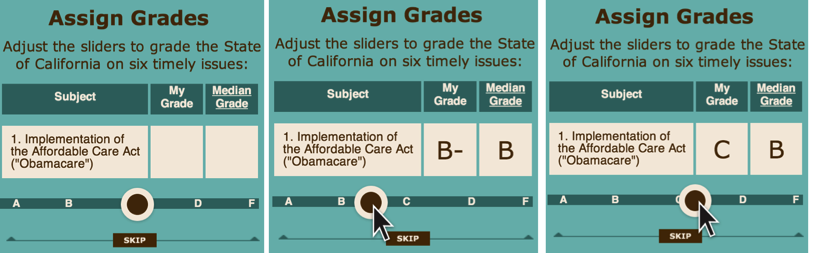
\includegraphics[width=\columnwidth]{../plots/grading-desc-1.png}
      \caption{After entering their rating, the median rating over all participants is revealed. Participants have the option to change their rating after seeing the median.}
      \label{grading-1}
\end{figure}

Upon release of the slider, the CRC reveals the median for that issue over all prior participants.
Even after the median is revealed the slider is still active and participants can change their ratings.
However, it is important to note that participants were not explicitly told that they could change their rating.
Another important observation is that participants who accessed the application at different times may have seen different medians as they were calculated based on the data up to that point.
We recorded the initial rating, the median that the participant observed, and any subsequent changes along with timestamps for each of the events. 
Rating all of the six issues was not mandatory and participant had the option to skip any of the issues.
To analyze this data, we mapped these 13 grade values linearly onto a scale from 0 to 1, with 1 being an A+ and 0 being an F.

\subsection{Notation}
Let $P$ denote the set of all participants.
For each participant $p_j\in P$, we associate a 3-tuple of ratings ($g_i[j]$, $m[j]$, $g_f[j]$) which represent the initial rating, median observed by the participant, and the final rating.
For each issue, we divided the participants into three subsets of $P$: ones who did not change their ratings $P_n$, ones who changed $P_c$, and ones who skipped the question $P_s$.
Our primary objective is to test the distributional properties of rating tuples from participants in $P_n$ compared to those in $P_c$.

To ensure that all participants in the set $P_c$ had an opportunity to see the median and then react, we filtered this group using the timestamps. 
The median appears in the interface with an animation whose completion time varied between devices, so we set a grace period of 3 seconds before 
we categorized the participant into set $P_c$.  

For consistency, we use the same notation to describe participants in the reference survey. We denote the set of reference survey participants as set $R$, and each participant is associated with a 3-tuple ($g_i[j]$, $m[j]$, $g_f[j]$). However, since the reference survey does not reveal the median $g_i[j] = g_f[j]$  and $m[j]$ is the hypothetical median of the prior participants (which is not shown).

\section{Analysis Phase}\label{ht}
In the analysis phase, we determine whether social influence bias is statistically significant by analyzing spread of ratings around the median for the participants that changed their ratings.
There are three principle challenges in testing this hypothesis.
The first challenge is that parametric significance tests comparing two sample means such as the two sample t-test and z-test are known to 
perform poorly for multimodal and discrete distributions.
Another significance test that is commonly applied to compare spreads of distributions is the F-test, which is also known to perform poorly for many non-normal distributions \cite{markowski1990conditions}.
Furthermore, this test is usually used to test the spread of data around the mean, which only in very special conditions, such as normal distributions, aligns with the median which is the parameter of interest in the CRC. 
The discreteness of our data leads to multi-modal distributions which are not optimal for these testing methods.

The second challenge is that there is a natural tendency for ratings to concentrate around the median even without a bias.
Consider the following participant behavioral model.
Suppose that participants are not accustomed to a slider-based input.
We can model the first rating that the participant leaves as uniformly randomly anywhere on the slider.
As the participant begins to understand how to use the slider, their use becomes more accurate, ultimately settling on a rating from our observed distribution of final ratings.
This model, the first rating is uniformly random and the second rating is a sample from the observed distribution, would result in a strong regression towards the median; even if there is no causal link with seeing the median.

Finally, the median $m_i$ changes as ratings arrive and thus can be different for each participant.
The median rating is calculated over all prior participants and thus is dependent on when the participant submitted their first rating.
In practice, the median will eventually converge for a large number of participants, but it would be incorrect to measure concentration around a final median.

To address these three challenges, we propose a nonparametric model based on the Wilcoxon statistic to test the hypothesis that the group of participants that changed their ratings are more tightly centered around the median value that those participants observed.
Our tests compare absolute deviations around the median for $P_n$, $P_c$, and $R$; which, as a relative comparison, controls for the natural tendency for ratings group around the median.
Furthermore, it is more robust to the effects of alternate models such as the one described in our second challenge in comparison to a direct test of correlation (see Section \ref{exp-robust}).
\subsection{Non-parametric Significance Test}
Recall that $P_n$ is the set of participants that did not change their ratings and $P_c$ be the set of participants that changed their ratings.
We define a set $X_c,X_n$ of absolute deviations from the observed median of the final rating for each group:
\begin{equation}
X_c = \{|m[j] - g_f[j]|\}\text{ }\forall j \in P_c
\end{equation}
\begin{equation}
X_n = \{|m[j] - g_f[j]|\}\text{ }\forall j \in P_n
\end{equation}
For the purposes of hypothesis testing, we ignore the sign of the deviation.
However, in Section \ref{changemod}, where we build a predictive model for the changes, we include the sign.

Now, for the set $X_c$, we calculate the Wilcoxon rank-sum statistic.
We assign a rank to each of the absolute deviations in the union set $\textbf{X} = X_c \cup X_n$ (ie. the largest change has rank 1 and the smallest has rank $|X_c \cup X_n|$.
For $X_c$, we sum the ranks of the deviations within its set:
\begin{equation}
W_c = \sum_{j \in P_c} R_j
\end{equation}

The \emph{Null Hypothesis} is that absolute deviations in $X_c$ are the same size as $X_n$. 
Under this null hypothesis $median(X_n) = median(X_c)$, the ranks will be evenly distributed between each group. 
Therefore, the null expected value and variance of $W$ is:
\begin{equation}
\mathbb{E}(W) = \frac{(|\textbf{X}| + 1)\cdot |X_c|}{2}
\end{equation}
\begin{equation}
var(W) = \frac{(|\textbf{X}| + 1)\cdot |X_c| \cdot |X_n|}{12}
\end{equation}
For the significance level $\alpha$, we can test the probability that our calculated $W_c$ comes from the null distribution.
In other words, the test calculates the probability that a random subset of users (ignoring the categorization $P_n$ and $P_c$) can have the observed difference in rank-sum values.
A significant result means that for the participants that changed their ratings the changed changes are more tightly centered around the median they observed.
For many distributions, the Wilcoxon statistic is more robust as it uses ranks rather than the actual values, making it more resilient to outliers.
Even in the case where the data is normally distributed, the optimal condition for the t-test, the relative efficiency of the Wilcoxon rank-sum statistic compared to the typically used t-statistic is $\frac{3}{\pi}=95.4\%$.
We trade off a small amount of efficiency in the normally distributed case, for increased efficiency and robustness in many non-normal distributions (eg. exponential $3\times$ more efficient).
Recommender system data is almost always collected from discrete inputs which are usually not normally distributed.

The same analysis can be used to test $X_c$ against the absolute deviations in the reference survey $X_r$
\begin{equation}
X_r = \{|m[j] - g_i[j]|\}\text{ }\forall j \in R
\end{equation} 
or for initial vs. final ratings in the change group $X_c'$:
\begin{equation}
X_c' = \{|m[j] - g_i[j]|\}\text{ }\forall j \in P_c
\end{equation}
\subsection{Quantifying Concentration of Ratings}
In addition to testing social influence bias, we can also estimate by how much the absolute deviations differ. 
The Wilcoxon statistic can be inverted to estimate a most likely \emph{shift parameter} $\Delta$, that is a shift $\Delta$ in the distribution of absolute deviations $X_c$ that maximally aligns them with $X_n$.
In other words, $X_c + \Delta$ is most supported by the null hypothesis (no social influence bias), or the distance from this hypothesis.
An intuitive interpretation of $\Delta$ is that it measures how much our deviations have to be increased so that the no social influence bias hypothesis is the most likely conclusion.
Since $X_c$ is a set of absolute deviations, $\Delta$ tells us how much more concentrated $X_c$ is than $X_n$ around the observed medians.
This parameter is relevant to the design of recommendation algorithms use similarity (eg. clustering or nearest neighbors), as it characterizes how much more on average are participants closer to the median.

We refer to \cite{lehmann2006nonparametrics} on the derivation of $\Delta$ and its confidence interval:
\begin{equation}
D = \{x_n[j] - x_c[i]\} \text{ } \forall i,j \in X_n, X_c
\end{equation}
\begin{equation}
\Delta = median(D)
\end{equation}
%\subsection{Discussion About the Grade Distribution}
%In Figure \ref{dist-1}, we show the distribution of absolute deviations for the Marriage Rights issue. 
%\begin{figure}[ht!]
%  \centering
%    \includegraphics[scale=0.40]{../plots/absolute-deviations.eps}
%      \caption{\textbf{TODO}}
%      \label{dist-1}
%\end{figure}
%We see that the distribution is multimodal and discrete. 
%Parametric tests such as the z-test and the t-test have been shown to have weaker statistical power in many families of multimodal distributions such as mixtures of Gaussians \cite{???}.
%Rank-based tests tend to be more robust to the multimodality and in fact don't depend on the actual values on the relative frequency of the ranks in the test set.


%\input{path_model.tex}
\section{Bias Mitigation}
\label{changemod}
In our learning phase, we collect rating triplets ($g_i[j]$, $m[j]$, $g_f[j]$), and in our analysis phase, we determine whether the triplets exhibit statistically significant social influence bias. 
In the mitigation phase, we propose two models: a correction model (infers the initial rating given a final rating and the median), and a prediction model (predicts final ratings given an initial rating and the median).
Once trained, the correction model can be applied to correct final grades collected without the triplet (either historical or post-learning).
The prediction model can be used to analyze properties of the social influence bias eg. are ratings above the median affected the same way as ratings below the median.

Previous work, suggests that social influence is not a homogeneous bias, namely, positive influences are different from negative influences.
In Muchnik et al. \cite{muchnik2013social}, they found that when they positively treated posts with higher up-vote counts it lead to a significant increase in the likelihood of additional up votes (32\% more likely). 
On the other hand, they argue negative treatments inspired correction behavior; where some participants wanted to correct what they felt was an incorrect score. 
They found that this also increased the likelihood of up-voting (88\% more likely); as opposed to the conforming response which would be increased down-votes.

These results suggest that the effects of viewing median ratings can be non-linear and are very context/question dependent.
Similar to the previous section where we applied non-parametric tests that did not make a strong assumption about the distribution of the data, we propose a information theoretic polynomial function search that does not make strong assumptions about the nature of the relationship.

\subsection{Correction Model}
Recall that $g_f[j]$ is the final rating for participant j, and $m[j] - g_i[j]$ is the difference between the median and the initial rating.
We want to find a polynomial function $f$ such that:
 \begin{equation} f(g_f[j]) 
 \approx m[j] - g_i[j]
 \end{equation}
Let $f\in \mathcal{P}^k$ be a polynomial of degree $k$.
The square loss of $f$, is the error in predicting $m[j] - g_i[j]$ from $f(g_f[j])$:
\begin{equation}
\mathcal{L}(X_c;f,k) = \sum_j ((m[j] - g_i[j]) - f(g_f[j]))^2 
\end{equation}
For a given $k$, the best-fit polynomial minimizes this square-loss:
\begin{equation}
f^*_k =\arg \min_f \mathcal{L}(X_c;f,k)
\end{equation}
For a given $k$, this problem can be solved with least squares.
To search over the space of polynomial models, we apply a well-studied technique called the Bayesian Information Criterion (BIC) \cite{schwarz1978estimating,burnham2002model}.
This technique converts the optimization problem into a penalized problem that jointly optimizes over the ``complexity parameter" $k$.
This penalty can be interpreted as bias towards lower degree models, in other words, an Occam's Razor prior belief. 
Cross-validation is an alternate method to empirically determine optimal model, and in practice, they give very similar results.
BIC, however, is derived through maximum likelihood estimate and is not an empirical estimate so the learned model has a notion of optimality conditioned on the BIC prior belief.

Thus, we reformulate the optimization problem in the following way to incorporate the BIC penalty:
\begin{equation}
\arg \min_{f,k} |X_c|\log(\mathcal{L}(X_c;f,k)) + k\log(|X_c|)
\end{equation}
The resulting optimal polynomial will tell how to correct a final rating to infer the initial one.
Let q:
\begin{equation}q(j) = m[j] - f(g_f[j])\end{equation}
the predicted initial grade, and this value can be the input to our recommendation algorithm.

\subsection{Applying the Corrections}
There are two ways in which we can apply the correction model to existing recommender systems data.
First, we can train our correction on all triplets, including ones that did not change, to get a correction that we can then apply to all ratings in the post-learning phase.
The second way is to estimate the probability that a rating is changed, and if that probability is above a threshold $\alpha$ (eg. 50\%) we can apply the correction.
With the second way, the correction model is only trained on those triplets where the initial rating is different from the final one.
To estimate this probability, we can apply a logistic regression model to predict whether or not a rating has been changed from all other ratings.
Let $c(i,j)$ be 1 if participant j changed his or her rating for issue i and 0 if not. 
Our feature vector is the vector of all final ratings for that participant $v[j]_f = [g_f^1[j],...,g_f^6[j]]$.
Then, we can apply this logistic regression model to estimate the probability that $c(i,j) = 1$, using the logistic function:
 \begin{equation}
 P[c(i,j) = 1] = \frac{1}{e^{-\beta^Tv[j]_f}}
 \end{equation}
We include results from both approaches in our experiments.

\subsection{Prediction Model}
For the prediction model, we make the dependent variable $m[j] - g_i[j]$ and the independent variable $g_f[j] - g_i[j]$.
We apply the polynomial regression with the BIC optimization as before, and find an optimal function $f$ such that \begin{equation}f(m[j] - g_i[j]) \approx g_f[j] - g_i[j]\end{equation}
$f$ is a function of the difference between the initial rating and the median, that predicts the change in rating.
This model allows us to reason about the nature of the social influence bias in the system.
For example, if $|f(x)| > |f(-x)|$ for $x > 0$, we know that ratings above the median lead to a larger rating change.
Additionally, $f'(x)$ tells us how the change varies as the observed difference with the median increases. 

\section{Results}
Use three datasets for which we have some ground truth. They are all small

Comparison: Pr* (Optimal single pipeline), RPr (All samples of EPS), RPr-50 (50\% of EPS samples), Pr- (worst pipeline), and baseline* (Jiannan's Crowder Clustering algorithm but using the best sequence of actions).

\subsection{Does Randomization Make Pipelining More Robust?}
Compare to best single pipeline, worst single pipeline, and current state of the art.
We should find that a randomized execution is much better than the worst and hopefully comparable to the best.
In some cases, it may be better than the best, but it should never be worse than the worst.

Dataset: MS Academic 
Operations: Filter and Deduplicate

Dataset: Yelp 
Operations: String Clean, City Format, Deduplicate

Dataset: Product 
Operations: identify sku if exists, string clean, Deduplicate

\begin{figure}[ht]
\centering
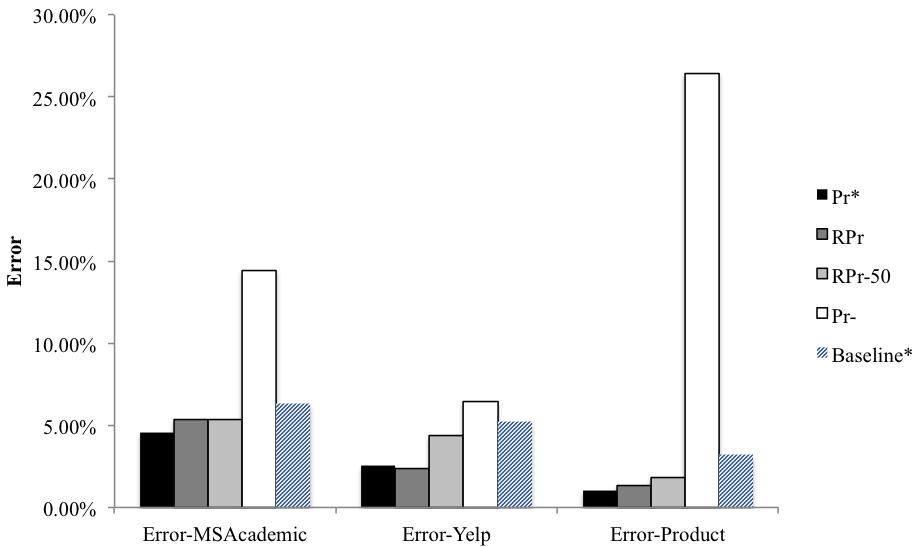
\includegraphics[scale=0.4]{fig1.png}
\caption{}
\label{exp:ms-academic-ranking}
\end{figure}

\subsection{How does this vary with random error in the operators?}
Should show that the more unreliable the data cleaning is the more that our approach benefits.

Introduce varying amount of random error (hashed so consistent between runs) into the ``city formatting" fix for the yelp dataset:

\begin{figure}[ht]
\centering
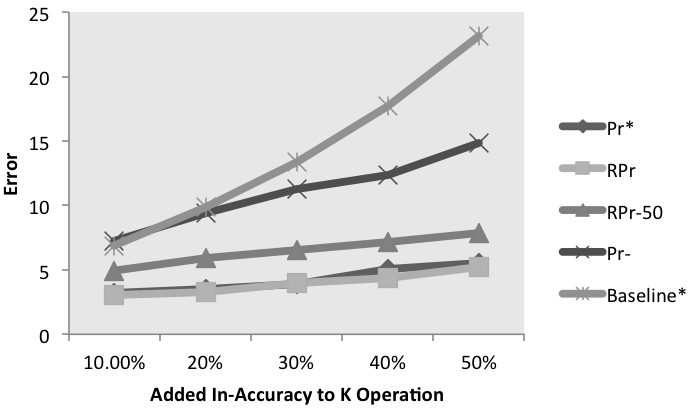
\includegraphics[scale=0.5]{fig2.png}
\caption{}
\label{exp:ms-academic-ranking}
\end{figure}

Introduce varying amount of random error (hashed so consistent between runs) into an extra dedup operation.

\begin{figure}[ht]
\centering
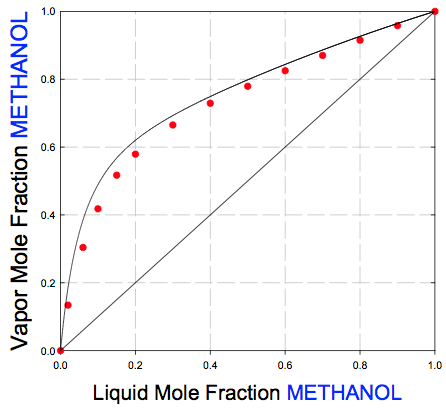
\includegraphics[scale=0.5]{fig3.png}
\caption{}
\label{exp:ms-academic-ranking}
\end{figure}

\subsection{Runtime-Accuracy Tradeoff}
Execute more samples and show how the accuracy improves.

\begin{figure}[ht]
\centering
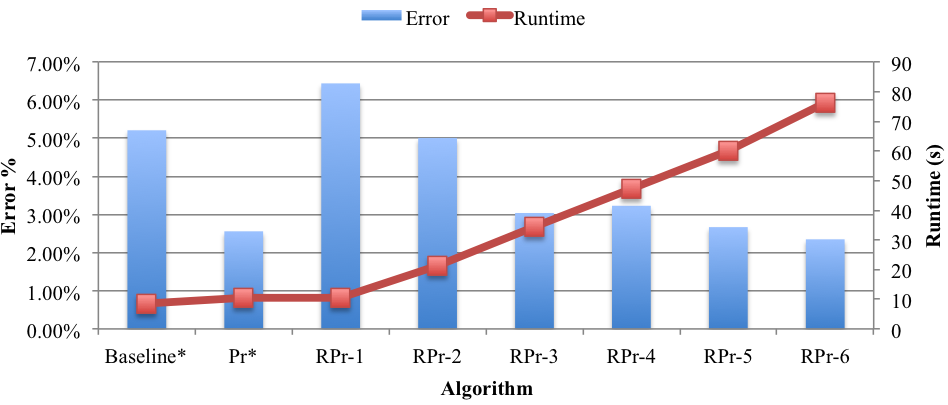
\includegraphics[scale=0.5]{fig4.png}
\caption{}
\label{exp:ms-academic-ranking}
\end{figure}


\subsection{Large-scale experiments}
Streaming correlation clustering. Show that at scale this technique can work and in a distributed environment.
In order to quantify the robustness of our methodology, we intend to run the algorithm on both synthetic and realworld datasets.
The synthetic dataset give us the ability to control the parameters while explore the state of possible responses.
However, a pitfall with such analysis is it's rather difficult to measure actual improvement over random fluctuations as well as the improvement may not be uniform across all tasks.
With experimentation on the real world datasets, we indent to first show the applicability of our method; and secondly determine whether results from our previous analysis extends to non-synthetic scenarios.



\vspace{-.5em}
\section{Conclusion and Future Work}\label{sec:con}
In this paper, we explore using sampling, integrated with data cleaning, to improve answer quality. We propose \saqpplus, a novel framework which only requires users to clean a sample of data, and utilizes the cleaned sample to obtain unbiased query results with confidence intervals.
We identify three types of data errors (i.e., value error, condition error and duplication error) that may affect query results, and develop \biascorrected and \sampleclean to estimate query results for the data with these errors.
Our analysis and experiments suggest that \saqpplus, which returns the better result between \biascorrected and \sampleclean, is robust to different magnitudes and rates of data errors, and consistently reports good estimate results.
%Moreover, \saqpplus can optimally satisfy user-specified cleaning-cost or result-quality constraints.
Our experiments on both real and synthetic data sets indicate that \saqpplus only needs to clean a small sample of the data to achieve accurate results, and furthermore the size of this sample is independent of the size of the dataset.
In particular, \sampleclean, which processes queries only on the cleaned sample, not only makes the query processing more scalable, but surprisingly may provide higher quality results than an aggregation of the entire dirty data (\alldirty).

To the best of our knowledge, this is the first work to marry data cleaning with sampling-based query processing.
%But, it is merely the tip of the iceberg.
There are many research directions for future exploration. 

\vspace{.25em}
{\noindent \bf Constrained Queries:} Now that we have quantified a tradeoff between cleaning costs and result quality, we can explore query results where users can specify a cost or quality constraint. For example, users may want to know that given a cleaning budget, what is the best result quality they can achieve? Or, given a quality constraint, how many samples they need clean to meet the constraint? 
In these constrained queries, we aim to answer with an optimal cost or most accurate result to meet the constraints.

\vspace{.25em}
{\noindent \bf Uncertain Cleaning Results:}  Our framework can return unbiased query results with respect to AllClean for a variety of different data cleaning approaches.
We are also interested in how we can incorporate uncertain or probabilistic cleaning processes into this framework.
For example, given a dirty record, could the data cleaning module specify a set of ranges for each attribute? 
We are interested in what guarantees, if any, we can achieve in such settings.

\vspace{.25em}
{\noindent \bf Complex SQL Queries:} Another important avenue of future work is to extend our framework to support more complex SQL queries such as join and nested SQL queries. There are some straightforward methods to implement these queries. For example, we can materialize the join result as a single table, and then apply our framework to the materialized table. But this could be very costly for large datasets, thus we need to explore more efficient implementations.
For a larger set of queries, it may not be possible to estimate their results with the CLT.
Thus, exploring empirical estimation approaches (such as bootstrapping) to our framework is another interesting future direction.

\vspace{.25em}
{\noindent \bf Sample Maintenance:} Finally, in real applications users may create multiple samples from the data.
Maintaining these samples for data updates is also very challenging and needs to be investigated.


\vspace{1.5em}

\fussy
{\noindent  \bf Acknowledgements.} {\small  The authors would like to thank Sameer Agarwal, Bill Zhao, and the SIGMOD reviewers for their insightful feedback. This research is supported in part by NSF CISE Expeditions Award CCF-1139158, LBNL Award 7076018, DARPA XData Award FA8750-12-2-0331, the European Research Council under the FP7, ERC MoDaS, agreement 291071, and by the Israel Ministry of Science, and gifts from Amazon Web Services, Google, SAP, The Thomas and Stacey Siebel Foundation, Apple, Inc., Cisco, Cloudera, EMC, Ericsson, Facebook, GameOnTalis, Guavus, Hortonworks, Huawei, Intel, Microsoft, NetApp, Pivotal, Samsung, Splunk, Virdata, VMware, WANdisco and Yahoo!.
}
\sloppy




%\end{document}  % This is where a 'short' article might terminate


%
% The following two commands are all you need in the
% initial runs of your .tex file to
% produce the bibliography for the citations in your paper.
{
\bibliographystyle{abbrv}
\fontsize{7.2pt}{7.6pt} \selectfont
\bibliography{sigproc}  % sigproc.bib is the name of the Bibliography in this case
}
% You must have a proper ".bib" file
%  and remember to run:
% latex bibtex latex latex
% to resolve all references
%
% ACM needs 'a single self-contained file'!
%
%APPENDICES are optional
%\balancecolumns

\balancecolumns
% That's all folks!
\end{document}
